\title*{System Software for Many-core \& Multi-core Architecture}

\author{Atsushi Hori, Yuichi Tsujita, Akio Shimada, Kazumi Yoshinaga,\\
Namiki Mitaro, Go Fukazawa, Mikiko Sato,\\
George Bosilca, Aur\'elien Bouteiller and Thomas Herault}
\institute{Atsushi Hori 
  \at RIKEN, 7-1-26 Minatojima-minamimachi, Chuo-ku, Kobe, Hyogo
  650-0047, JAPAN\\
  \email{ahori@riken.jp}
\and Yuichi Tsujita
  \at RIKEN, 7-1-26 Minatojima-minamimachi, Chuo-ku, Kobe, Hyogo
  650-0047, JAPAN\\
  \email{yuichi.tsujita@riken.jp}
\and Akio Shimada
     \at Hitachi, Ltd., Research\&Development Group, 292,
     Yoshida-cho, Totsuka-ku, Yokohama, Kanagawa, 244-0817, JAPAN,
     \email{akio.shimada.ht@hitachi.com}
\and Kazumi Yoshinaga
     \at Clotho Co., Ltd., Where ???
     \email{kazumi@kuromi-love.com}
\and Namiki Mitaro
     \at Tokyo University of Agriculture and Technology, 
     Naka-cho, Koganei-shi, Tokyo 184-8588, JAPAN,
     \email{namiki@cc.tuat.ac.jp}
\and Mikiko Sato
     \at Tokai University, School of Information and Telecommunication
     Engineering, Department of Embedded Technology, 
     2-3-223 Takanawa, Minato-ku, Tokyo 108-8619, JAPAN\\
     \email{mikiko.sato@tokai.ac.jp}
\and Go Fukazawa
     \at Yamaha Corp., 10-1 Nakazawa-cho, Naka-ku, Hamamatsu,
     430-0904, JAPAN\\
     \email{go.fukazawa@fzawa.net}
\and George Bosilca
     \at Innovative Computing Laboratory, University of Tennessee,
     Suite 203 Claxton, 1122 Volunteer Blvd., Knoxville, TN37996, USA,
     \email{bosilca@icl.utk.edu}
\and Aur\'elien Bouteiller
     \at Innovative Computing Laboratory, University of Tennessee,
     Suite 203 Claxton, 1122 Volunteer Blvd., Knoxville, TN37996, USA,
     \email{bouteill@icl.utk.edu}
\and Thomas Herault
     \at Innovative Computing Laboratory, University of Tennessee,
     Suite 203 Claxton, 1122 Volunteer Blvd., Knoxville, TN37996, USA,
     \email{herault@icl.utk.edu}
}

\authorrunning{A. Hori, et al.}
\maketitle 

\abstract{
blablabla
}

\section{Overview and Background}

The goal of this project was to develop OS technologies needed for
post-peta scale machines in the future under the assumption of such
KNC-like architecture would dominate. The goal of this project was to
develop key software technologies required for the post-peta scale
computers. There were 4 research topics in this project;

\begin{itemize}
\item OS technologies for heterogeneous architecture
\item Lightweight thread
\item Scalable I/O
\item Fault mitigation
\end{itemize}

This project was started from April 2011 and ended March 2016. When
this project was started, the first commercial many-core CPU, Intel
Knights Corner (known as KNC)\cite{overview-xeon-phi}, became
available and many people 
believed it was the dawn of many-core era. KNC was designed as a
co-processor and it needed a many-core CPU to be attached with. From
the view point of OS research, this heterogeneous CPU architecture was
new because an OS ran on each CPU, unlike the other co-processor
architectures such as GP-GPU or vector processing unit (e.g.,
ClearSpeed) where no (explicit) OS ran on those co-processors. 

The performance improvement of applications which have dynamic
workload is a big concern for the coming post-scale era. Lightweight
multithread is thought to be the answer for this kind of
applications. We proposed a novel technique for this topic.

I/O has been a headache in the long history of HPC. We focused on the
collective I/O in MPI and proposed several optimization techniques to
improve I/O performance.

Fault mitigation has been a big concern as supercomputers are scaling
up. In this project, we proposed two techniques; one is a parallel
execution environment in which a process failure can be mitigated, and
another is the technique how user programs can survive from the
failure by using spare nodes.

\section{OS Technologies for Heterogeneous Architecture}

The widely-used in-node parallel execution models are
multi-process model (e.g., MPI) and multi-thread model (e.g.,
OpenMP). The multi-process model has the problem when to communicate
with the others because each proceee has its own virtual address space
and shared memory is often used to for inter-process
communication and this cannot avoid the 2-copy to exchange data
between processes. The multi-thread model has the non-negligible  
overhead of mutual-exclusion on shared variables. Both overheads
become more striking when the number of cores increases. 

To have the best of the two worlds; multi-process and multi-thread,
the third execution model has been proposed and implemented. SMARTMAP
is to pack processes into one virtual address space, but SMARTMAP only
runs on Kitten OS\cite{Brightwell:2008:SOS:1413370.1413396}. MPC
allows threads to have privatized variables, but MPC heavily depends
on a language processing system and it requires special language
processing system\cite{pjn2008}. We
decided to develop our own system to implement the third execution
model. This is called {\em Partitioned Virtual Address Space (PVAS)}
implemented by the patched Linux kernel. Its details is explained in
the next subsection. 

PVAS provides the efficient parallel execution mode on many-core
architectures. However, our final target architecture is heterogeneous,
where many-core CPU and multi-core CPU are connected by an I/O
bus. Each CPU has its own physical memory. An OS runs
independently on each CPU. On KNC, Intel provides the SCIF to
communicate between the KNC process and host 
process. Unfortunately, its communication performance was not so
good (shown in Subsection~\ref{sec:mpvas}). Our proposed solution to
this is the extension of PVAS to pack processes on KNC and processes
on host processor into one virtual address space so that every
process can access the data of the other processes regardless of the
CPU on which processes are running. This scheme was called
{\em Multiple-PVAS (MPVAS)} and more efficient communication than Intel
provided SCIF could be achieved. 

\subsection{Partitioned Virtual Address Space}\label{sec:pvas}

Basically, a process has an isolated virtual address space, and it
cannot access the data in the other process. Shared memory technique
is widely used to implement inter-process communication in HPC. Shared
memory is a special memory region which physical memory region is
shared between processes and the data in the shared memory region can
be accessed from the processes sharing the memory region. However,
when to communicate between two processes, sender process write a data
into the shared memory segment and receiver process read the data in
the shared memory segment. Thus, two memory copies take place and this
memory copy overhead hinder the parallel execution.

Each process has its own virtual address space so that the process is
guaranteed not to be interfered by the other processes. Let's assume
that there are two processes connected by a pipe. If a sender process
dies for some reason then the receiver process is killed by the {\tt
SIGPIPE} signal.  Even if the {\tt SIGPIPE} signal is ignored, then the
receiver process might be blocked forever for receiving data, since
there is no process to send data to the receiver process. Thus,
communicating processes can be said to share the same fate. 
In the coming many-core era, the intra-node communication will be more
frequent. Therefore the development of efficient intra-node
communication is important.

\begin{figure}[ht]
\begin{center}
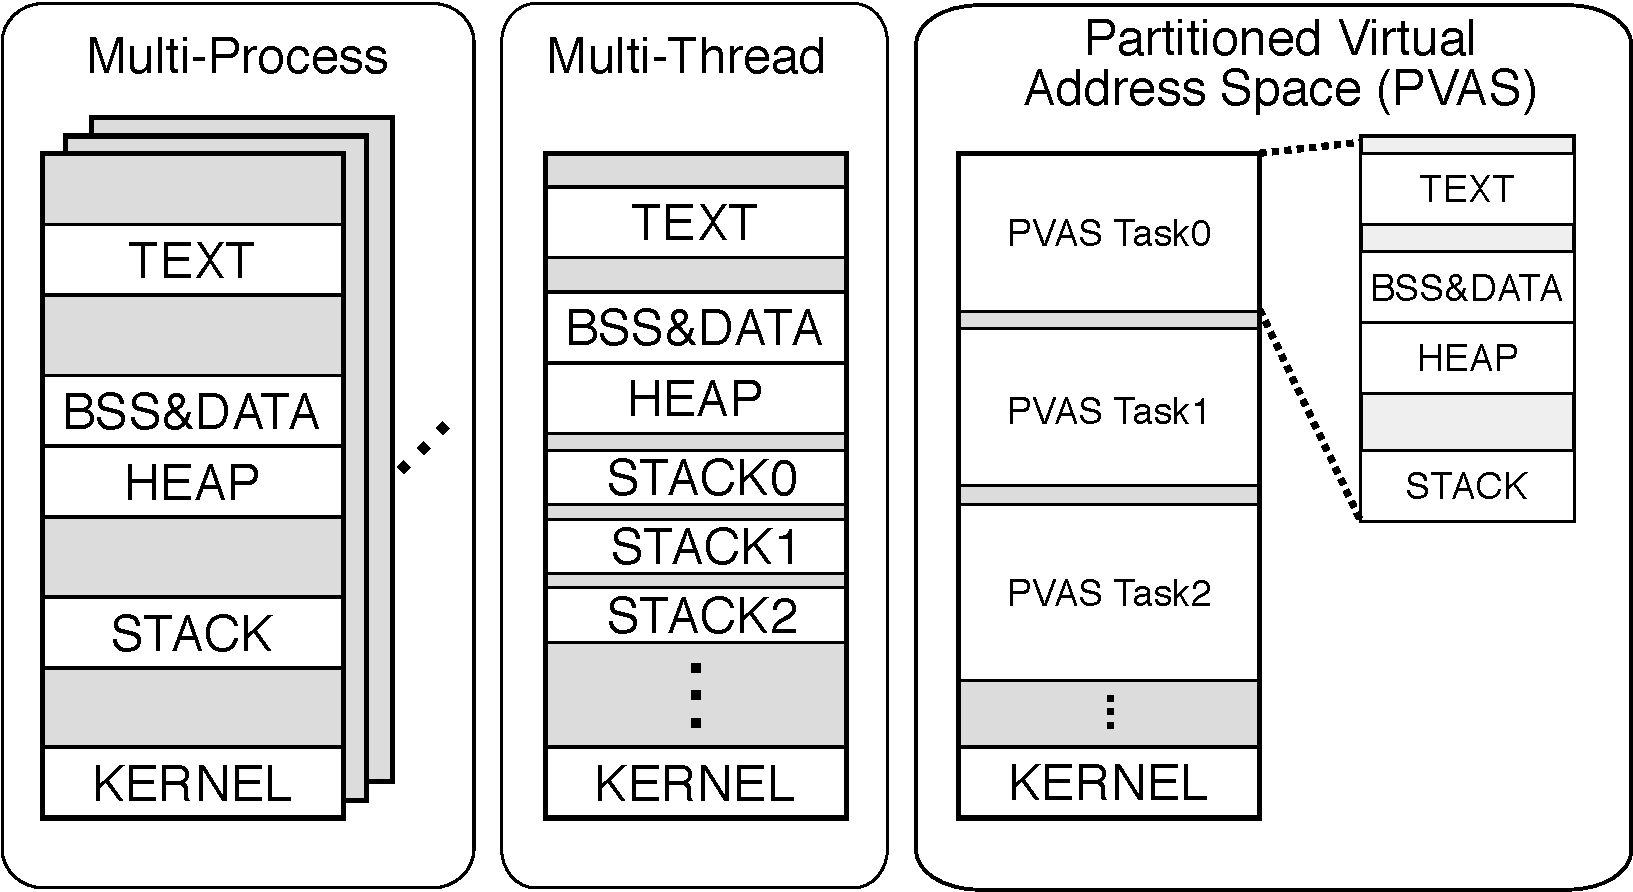
\includegraphics[width=0.8\columnwidth]{Figs/PVAS.pdf}
  \caption{Address Maps of Multi-Process, Multi-Thread and PVAS}
  \label{fig:pvas-map}
\end{center}
\end{figure}

If all communication processes share the same virtual address space,
then the data owned by a process can be accessed by the other
processes without incurring the overhad of 2-copy. This is the idea of
PVAS\cite{110009850784,Shimada:2014:ECC:2642769.2642790,SHIMADA:PGAS12,Shimada:2013:PNT:2489068.2489075,shimada-thesis}. The
virtual address space is  
firstly partitioned and process occupies one of the partitions. To
implement PVAS, the Linux OS kernel is patched. 

\begin{figure}[ht]
\begin{center}
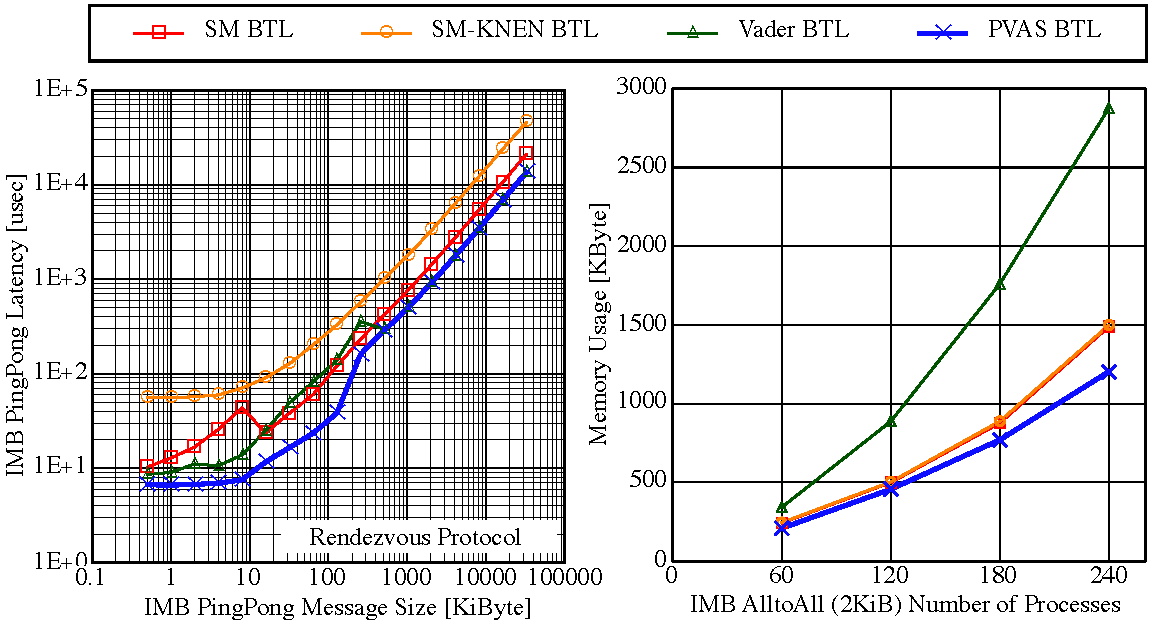
\includegraphics[width=0.95\columnwidth]{Figs/PVAS-BTL.pdf}
  \caption{IMB PingPong Latency (Left) and Memory Consumption (Right)}
  \label{fig:pvas-btl}
\end{center}
\end{figure}

Figure~\ref{fig:pvas-btl} shows the communication performance
comparisons among shared memory denoted as ``SM BTL,'' KNEM (a kernel
assisted 1-copy messaging) denoted as ``SM-KNEM BTL,'' XPMEM (allows
process to expose a memory region to be accessed by the other process)
denoted as ``Vader BTL'' and PVAS denoted as ``PVAS BTL.'' This
evaluation was carried out on Xeon (E5-2650v2, 2.60GHz). The left
graph shows the PingPong latency measured by using IMB benchmark, and
the right graph shows the system-wide memory usage of IMB Alltoall
communication. As shown in those graphs, the intra-node communication
using PVAS exhibits the lowest latency and the least memory usage.

In MPI point-to-point communication, MPI datatypes which is an
expression of non-contiguous data layout can be specified in
the send function and the receive function. Since datatype information
is local and the sender process has no knowledge on the datatype on receiver
process in most MPI implementations using multiprocess model. In the
current MPI implementations, if a sender 
wants to send a non-contiguous data to a receiver, firstly the sender
packs the non-contiguous data and then send the packed data to the
receiver. And on the receiver process, the packed data is
unpacked. Thus, costly message 2-copy must take place.

With PVAS, however, the sender process can take a look at the datatype
information on the receiver process. This is because the sender 
process and the receiver process share the same virtual address space in
PVAS. And non-contiguous messages can be sent with
1-copy according to the datatypes of sender and
receiver. \cite{shimada-thesis} reported 20\% improvement with {\tt 
ft2d\_datatype} benchmark\cite{mpi-ddt-benchmark}.  

\subsection{Heterogeneous Extension of PVAS}\label{sec:mpvas}

On KNC, there are two sets of CPU and memory and these are connected
by the PCIe bus. Independent OS runs on each CPU. The multi-core CPU
has a fewer number of fast cores and the many-core CPU has a large
number of slow cores. Applications having large parallelism can
exploit the power of many-core. When an application running on
many-core CPU tries to send a message using MPI, for example, then MPI's
complex protocol which is very hard to parallelize must be
handled by the slow many-core CPU. This can add extra latency when
compared with the case of using multi-core CPU.

The idea here is to delegate the heavy protocol handling from
many-core CPU to multi-core CPU so that the complex MPI protocol can
be handled by the faster multi-core CPU. The key technology here is
the low-latency delegation mechanism from many-core CPU to multi-core 
CPU, and vice versa. Generally speaking, this idea can be applied not
only MPI but many situations where required parallelism of a
computing phase is very different from the other phase.

\begin{figure}[ht]
\begin{center}
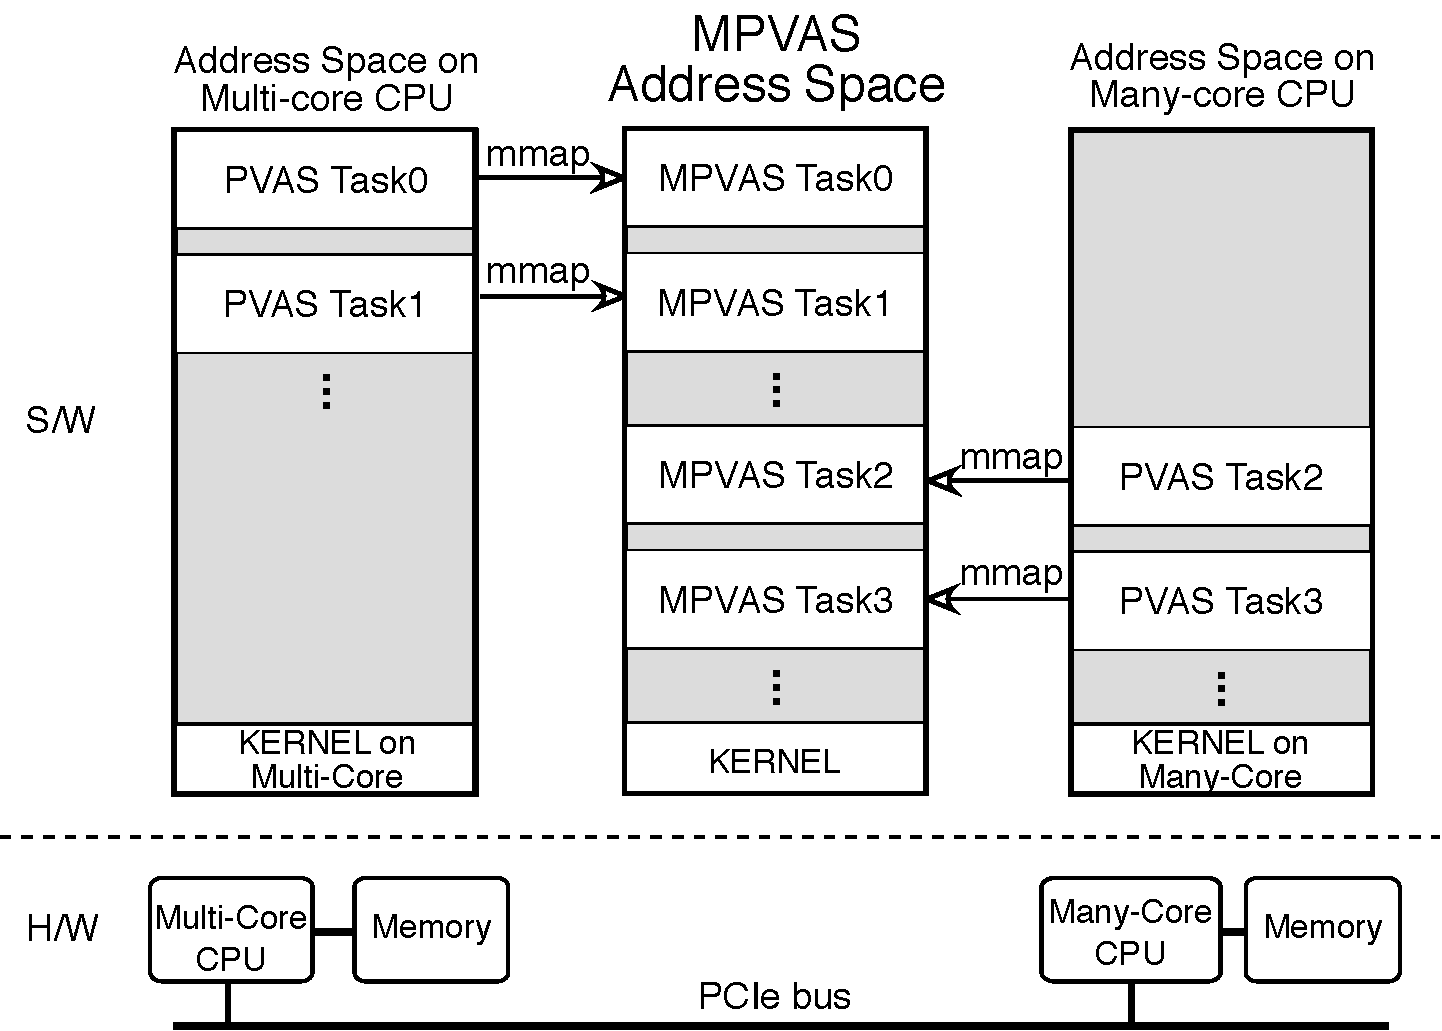
\includegraphics[width=0.8\columnwidth]{Figs/MPVAS.pdf}
  \caption{Multiple PVAS}
  \label{fig:mpvas}
\end{center}
\end{figure}

Multiple-PVAS (MPVAS) was designed for such purpose. The processes
running on many-core CPU and the processes running on multi-core CPU
are mapped into one virtual address space
(Figure~\ref{fig:mpvas})\cite{fukazawa-thesis}. In MPI, to 
send a message from a process on many-core CPU, the send request is
passed to the process running on multi-core CPU, and then the request
is processed on multi-core CPU. Since the data to be sent can be
accessed by the multi-core process, there is no need of copying it. 

\begin{figure}[ht]
\begin{center}
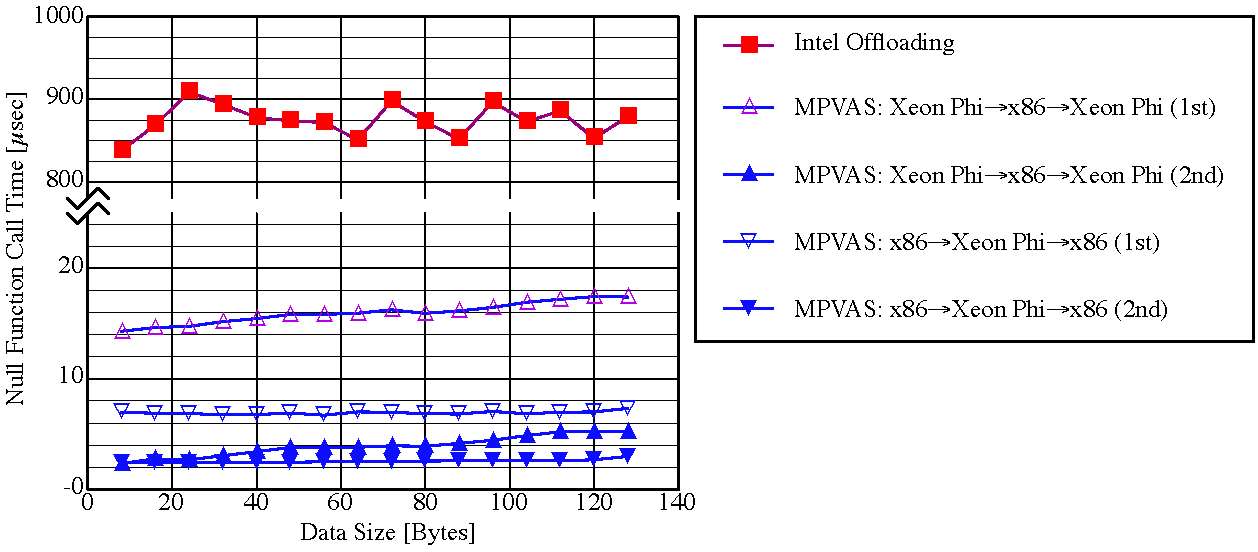
\includegraphics[width=0.95\columnwidth]{Figs/MPVAS-TAT.pdf}
  \caption{Inter-CPU Offloading Latency (KNC)}
  \label{fig:mpvas-tat}
\end{center}
\end{figure}

Figure~\ref{fig:mpvas-tat} shows the latency of RPC between many-core
(E5-2650v2, 2.60GHz) and multi-core (Xeon Phi 7120P). X-axis shows the
payload length and Y-axis shows the latency. As shown in this figure,
the latency of using the offloading mechanism provided by Intel is
several order of magnitude slower. Fukazawa reported that the MPI
latency with this delegation mechanism is almost halved compared with
the one using only many-core CPU\cite{fukazawa-thesis}. 

\section{Lightweight Thread}

PVAS can be used to implement a novel execution model. In PVAS,
processes are mapped in the same virtual address space. Here, each
process has an associated OS kernel thread to run in parallel. There
can be PVAS processes having no associated OS kernel thread and there
can be PVAS processes having OS kernel thread. Assume PVAS process $A$
has no OS kernel thread and PVAS process $B$ has OS kernel thread. The
OS kernel thread of $B$ can switch to $A$ at user level by calling
the {\tt swapcontext()} or {\tt setcontext()} Glibc function. This
mechanism is very similar to the one of user-level thread. However,
each PAVS process may have different program and do have privatized
variables, unlike user-level thread. The time for the context
switching of ULP is almost equal to the time of user-level thread. 
We named this {\em User-Level Process (ULP)}
because PVAS processes behave like a process\cite{110009850784}.

If MPI processes in a node were implemented by using ULP and they were
oversubscribed by having more number of MPI processes than the number
of CPU cores, then those MPI processes can be switched from one to
the other in a fast way. 

\section{Scalable I/O}

The current optimization technique of collective MPI-IO\cite{romio} is
based on Two-Phase I/O\cite{two-phase}, where the scattered I/O
requests on compute nodes are 
sorted according to the parallel file offset and then actual I/O
requests are sent to I/O servers. This technique is very effective
because the smaller I/O requests on compute nodes are gathered on
aggregator nodes so that larger I/O requests can be sent to I/O
servers. 

In general, not limited to HPC, it is the file servers nature that a
number of simultaneous I/O requests can degrade its performance. To
prevent this, I/O throttling technique was proposed. In the Two-Phase
I/O, a number of I/O requests are also sent to I/O servers. Our first
idea is to throttle the number of request to the IO servers to get
higher performance. There is another bottleneck in Two-Phase
I/O. All-to-all like communication between user processes and
aggregator processes to sort and merge the users' I/O requests takes
place. If the I/O requests to the server are throttled, then this
all-to-all-like communication can also be throttled. Consequently, the
communication bottleneck can be relaxed. Thus, the flow  
of the I/O requests from user process to I/O servers can be done in a
way of step-wise pipeline to level the loads of the communication
network and I/O servers.

The optimization method is named {\em EARTH} which includes the above
step-wise communication, throttling to the I/O servers,
striping-aware data blocking and distribution, and 
optimized allocation of the aggregator processes to decrease the message
congestion in communication network. Figure~\ref{fig:earth} shows the
write bandwidth on the K computer comparing the original MPI-IO and
EARTH optimized MPI-IO. In the EARTH cases, the number of requests at
each step of the step-wise pipeline is also varied. As shown in this
figure, EARTH performs more better when the number of processes
increases. 

\begin{figure}[ht]
\begin{center}
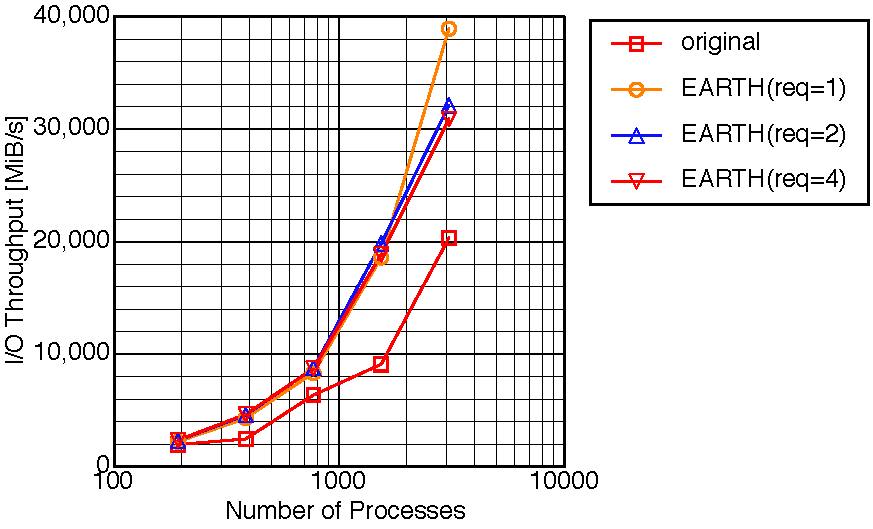
\includegraphics[width=0.95\columnwidth]{Figs/K-HPIO.pdf}
  \caption{HP-IO Write Performance (the K computer)}
  \label{fig:earth}
\end{center}
\end{figure}

\section{Fault Mitigation}

Checkpointing is a well-known technique to recover from a
failure. However, its cost can be very high and the fault mitigation
becomes the hot topic in the fault tolerant research field. User-Level
Fault Mitigation (ULFM) which is a user-level 
library for a parallel program to survive from a process failure is
gathering the attentions as a technique of fault mitigation. In this
project, a technique to improve the performance of ULFM was developed.
The implementation of ULFM is not easy. The signal of a process
failure must be propagated to the other processes to reach a consensus
of the failure. Another process failure may happen during the
propagation and consensus protools. ULFM must survive from any
process failure that can happen at any time. In the next subsection,
an optimization technique for ULFM to be more efficient is explained. 

Since ULFM provides the way where user program can handle process
failure events. It is up to the user program how to handle such
situation. Having spare nodes to replace failed node is considered to
be effective, however, study on the spare nodes is not active so far. We
focused on this issue and propose how to allocate spare nodes and how
failed nodes should be replace by the spare nodes. 

\subsection{User-Level Fault Mitigation (ULFM)}

\subsubsection{Conceptual Design}

The main goal of the
ULFM\cite{Herault:2015:PSC:2807591.2807665,Bouteiller:2015:PBI:2802658.2802668,doi:10.1177/1094342013488238}
approach remained unchanged over this 
period: define a minimal set of features to notify application
processes about failures, and allow the user to interrupt the normal
behavior of his application and to restore communication capability
after process failures. Exchanges with developers of MPI applications
who envision to introduce resilience in their codes, or who have tried
to do so using the ongoing ULFM specification, as well as fruitful
discussion in the MPI Forum, mainly inside the Fault Tolerance Working
Group and in plenary sessions, have highlighted few opportunities for
improvements in the ULFM specification. Ambiguities in the proposed
text have been removed, and replaced by a clearer description of the
required behavior. The RMA chapter has been entirely rewritten, to
account for the changes in the RMA chapter introduced in the version 3
of the MPI standard. The {\tt MPI\_Comm\_shrink()} and {\tt
MPI\_Comm\_agree()} routines, 
which are part of the Fault Tolerance extensions, have been
simplified, allowing for a more diverse usage. Non-blocking versions
of some of these constructs have been also added, to allow for more
flexible recovery strategies.

\subsubsection{Implementation}

In same time as improving the concepts design, we wanted to provide a
decent implementation that can be used by interested parties for their
own research and developments. The first part of the award period was
dedicated to providing correct, but non necessary efficient and
scalable, support for all concepts. In parallel we advanced on the
theoretical side by developing all the necessary tools and algorithms
to design and implement more scalable versions of the needed concepts.

More specifically, the last year of the project has been almost
entirely focused on advancing on the performance side of the two major
operations proposed for the handling of the faults (revocation and
agreement), and on promulgating the extension to the MPI standard to
the users communities. In same time, a significant effort has been
done to improve the code quality of the available implementation, in
order to provide a stable, efficient and portable implementation to
the user communities.

Similarly to past years, exchanges with developers of MPI applications
who envision to introduce resilience in their codes, or who have tried
to do so using the ongoing ULFM specification, as well as fruitful
discussion in the MPI Forum, inside the Fault Tolerance Working Group
and in plenary sessions, have highlighted a few places for
improvements in the ULFM specification. The main goal of the ULFM
approach remains unchanged: define a minimal set of features to notify
application processes about failures, and allow the user to interrupt
the normal behavior of his application and to restore communication
capability after process failures. Ambiguities in the proposed text
have been removed, and replaced by a clearer description of the
required behavior. The RMA chapter has been entirely rewritten, to
account for the changes in the RMA chapter introduced in the version 3
of the MPI standard. The {\tt MPI\_Comm\_shrink()} and {\tt
MPI\_Comm\_agree()} routines, which are part of the Fault Tolerance
extensions, have been simplified, allowing for a more diverse usage.

\begin{figure}[ht]
\begin{center}
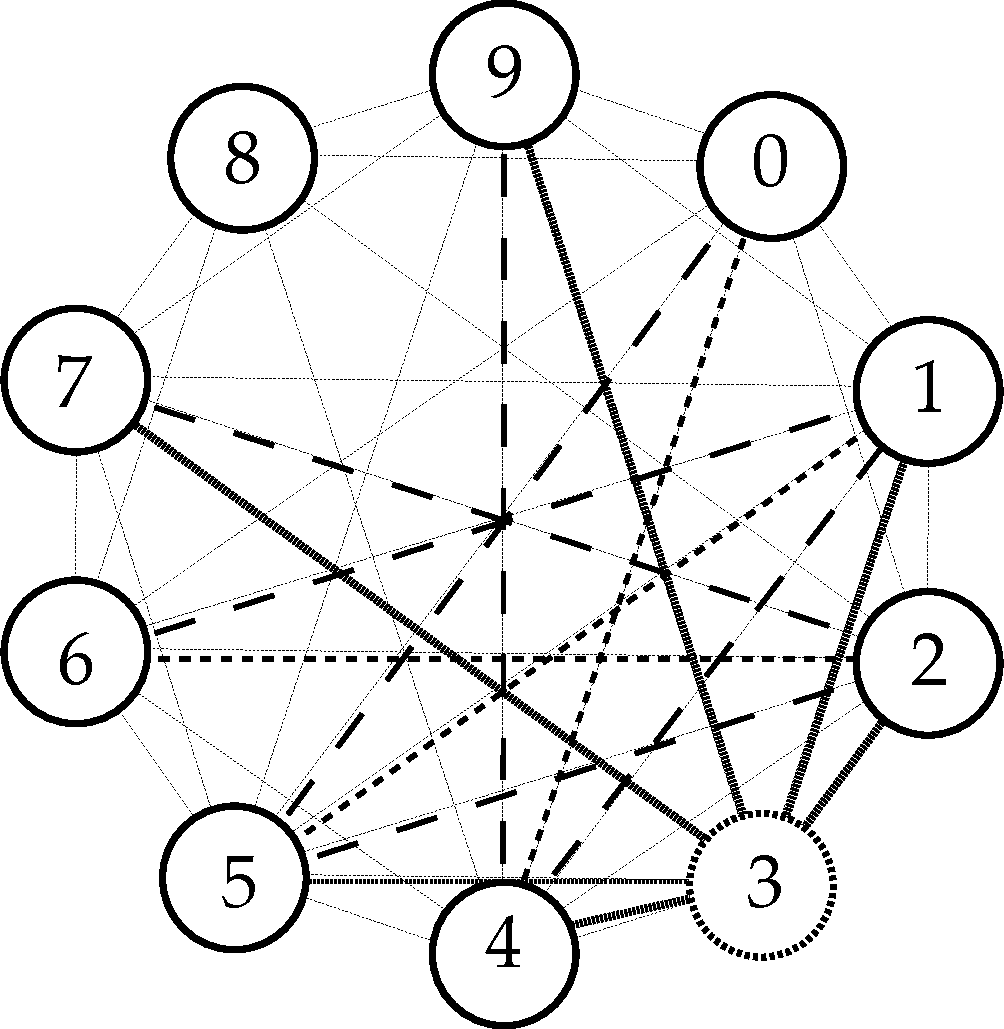
\includegraphics[width=0.4\columnwidth]{Figs/BinomialGraph.pdf}
  \caption{Binomial Graph Topology}
  \label{fig:binomial-graph}
\end{center}
\end{figure}

On the implementation front, the {\tt MPI\_Comm\_revoke()} and {\tt
MPI\_Comm\_agree()} 
operations have been the focus of our efforts for this year. These two
routines are critical to the efficiency of a resilient code, and are
by nature costly because they need to be fault-tolerant
themselves. {\tt MPI\_Comm\_revoke()} is provided to the user to notify
(asynchronously) all processes belonging to a communicator that an
exception happened, and to stop the normal execution flow (e.g. to
trigger a collective repair of the communicator). At the conceptual
level, it implements a form of reliable broadcast: if one process
receives such revoke notification, all processes of the communicator
must receive one. Because failures happening during the revoke
operation can introduce messages loss, the protocol that implements
the revoke operation must be fault-tolerant, and ensure that if one
notification is delivered, all notifications are delivered. The first
implementation of the revocation was done at the Runtime Environment
(RTE) level, over the Out-Of-Band (OOB) network. This implementation
was not fault tolerant and required a large number of messages
($O(N2)$). We redesigned the algorithms integrating research in
resilient graph topologies and successfully improved not only the
resilience and performance of the revocation algorithm but also the
impact on the network infrastructure and the number of messages. The
final algorithm that we will be delivered with ULFM is based on the
Binomial Graph topology (Figure~\ref{fig:binomial-graph}). This graph
minimize the number of 
messages and the degree of the graph, while providing a strongly
resilient topology, that can only be bipartite by the sudden
disappearance of more than half of the processes. Moreover, the new
algorithm is implemented at the BTL level, and takes advantage of the
fast network interconnect available on most of the HPC clusters.

\begin{figure}[ht]
\begin{center}
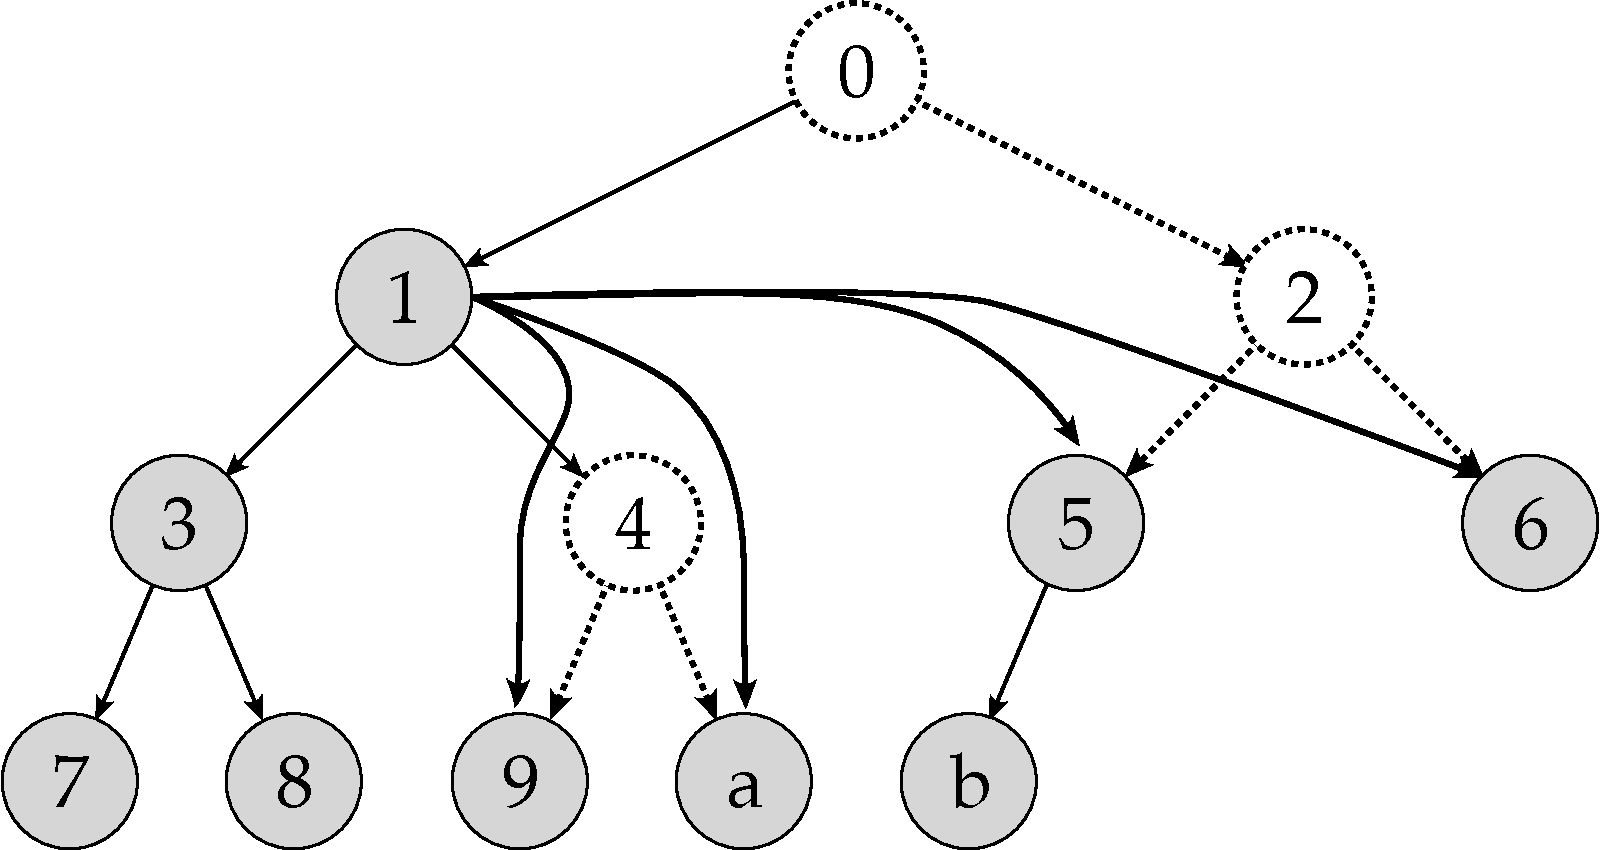
\includegraphics[width=0.6\columnwidth]{Figs/DynamicTopology.pdf}
  \caption{Example of Dynamic Topology}
  \label{fig:dynamic-topo}
\end{center}
\end{figure}

The {\tt MPI\_Comm\_agree()} routine was also relying, for parts of its
services (namely the all-reduce tree maintenance) on messages at the OOB
level. The overhead imposed by the OOB mechanism has been hindering
the performance and scalability of the agreement. We completely
reworked the agreement to use directly the fast network communication
infrastructure available in Open MPI (namely the BTL). This step
provided a significant boost in terms of performance of the agreement
algorithms. However, this highlighted few implementation issues with
quadratic search involved in the original algorithms (due mainly to
the MPI semantics of translating ranks between communicators). As a
result, we decided to redesign the agreement implementation from the
ground up. Dynamic topologies have been introduced, topologies that
remains optimal as long as no new processes disappear, and that are
updated upon a successful completion of an agreement (due to the
semantic of the agreement itself a consensus on the dead processes is
established during the agreement, allowing for a consistent global
view of the alive processes). This topology is described in the figure
above (Figure~\ref{fig:dynamic-topo}). The important change is the
orange lines, which 
represent the new connections that are established to cope with the
discovery of dead processes (signaled by the red dashed line). These
lines connect a process to the leftmost ancestor still alive, and
count for one of the most costly, but critical, operation during the
agreement. Without going in too much details, we have designed a new
consensus algorithm named Early Returning Agreement, with a worst case
cost of $\sum{f} = 1..F(\log(P-f))$ where $F$ is the number of fault discovered
during a single agreement and $P$ is the total number of processes.

Moreover, users reports signaled recurring corner cases in the
previous agreement implementations, where the agreement routine was
unable to provide its service because of the presence of failures. We
wrote a reference implementation of the agreement, based on an
existing Early Termination Agreement protocol, which work in
asynchronous all-to-all phases, ensuring a correct result in any
possible failure scenario. In addition to this reference
implementation, we initiated works on more efficient implementations,
which will take advantage of the high resilience property of the
Binomial Graph, to reduce the number of messages while still providing
the insurance of safe agreement despite failures in most situations.

\subsection{Spare Node Substitution}

This subsection considers the questions of how spare nodes should be
allocated, how to substitute them for faulty nodes, and how much the
communication performance is affected by such a substitution.
The third question stems from the modification of the rank mapping by
node substitutions, which can incur additional message collisions.
In a stencil computation, rank mapping is done in a
straightforward way on a Cartesian network without incurring any
message collisions. However, once a substitution has occurred, the
node-rank mapping may be
destroyed. Figure~\ref{fig:message-collisions} shows such an
example. In this case, the failed node substitution results in having
at most 5 message collisions (in the dashed circle). When two message
collides, then the latency is doubled. Thus, the number of message
collisions should be as low as possible.

\begin{figure}[ht]
\begin{center}
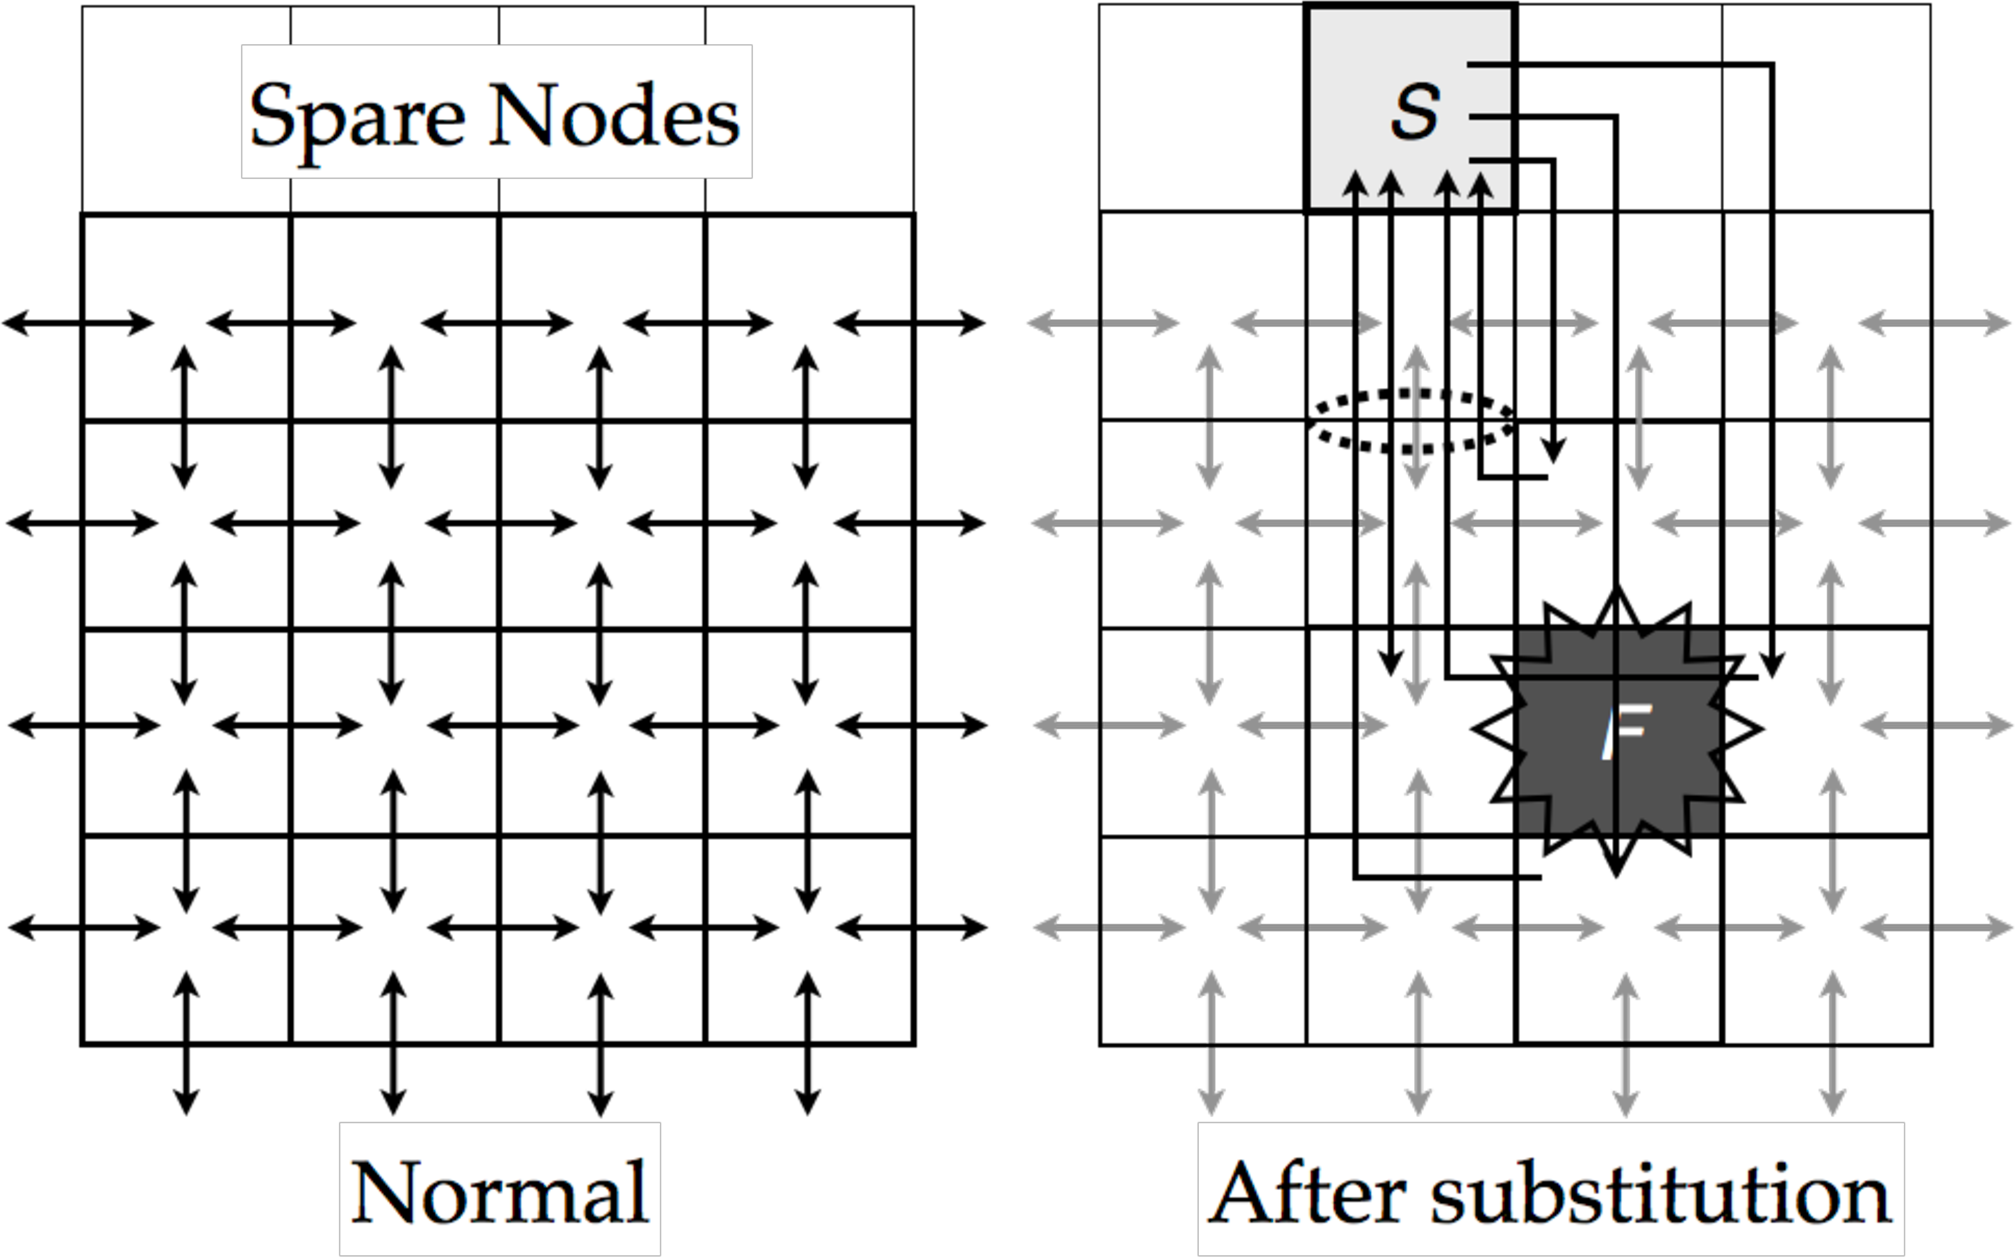
\includegraphics[width=0.6\columnwidth]{Figs/MessageCollisions.pdf}
  \caption{Message Collisions}
  \label{fig:message-collisions}
\end{center}
\end{figure}

The number of message collisions depends on the spare node allocation
and how the failed node is substituted. Here, network topology is
assumed to be Cartesian of any order. Although the substitution idea
proposed here can be applied to Cartesian having any order, the
explanations are mostly using 2D network topology, due to the
simplicity. 

\begin{figure}[ht]
\begin{center}
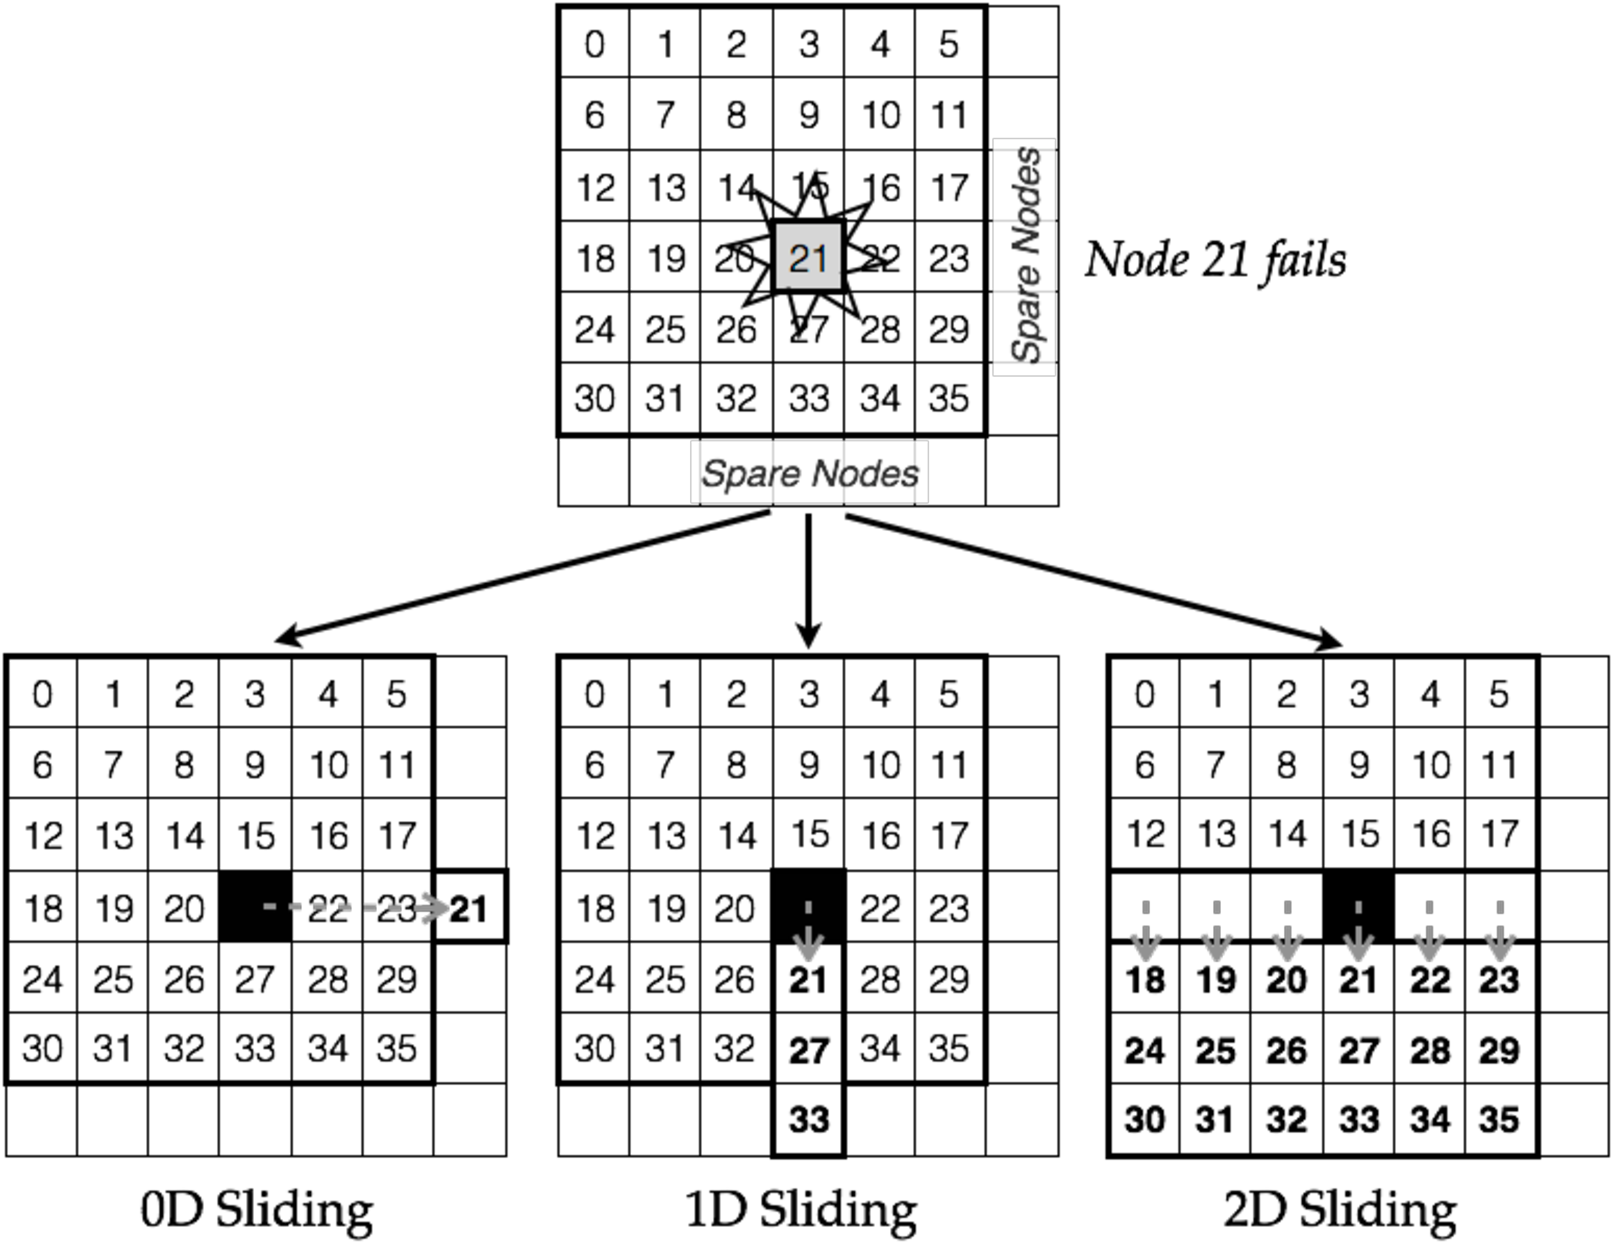
\includegraphics[width=0.95\columnwidth]{Figs/SlidingSubstitution.pdf}
  \caption{Sliding Methods}
  \label{fig:sliding-methods}
\end{center}
\end{figure}

Figure~\ref{fig:sliding-methods} shows how the failed node is
substituted in this proposed way. In this example, spare nodes are
allocated at the edges of the 2D node space. The {\em 0D sliding}
method is most simple one, just replace the failed node with a spare
node which is located to the nearest Manhattan distance from the
failed node. In {\em 1D sliding} method, firstly the spare node having
the same X-akis or Y-axis is chosen and the nodes between the failed
node and the spare node are shifted. In {\em 2D sliding} method, all
nodes having the larger X-axis or Y-axis location are shifted. In
general, the sliding method can be extended up to {\em $N$D sliding},
where $N$ is the dimension of a Cartesian topology network.

\begin{figure}[ht]
\begin{center}
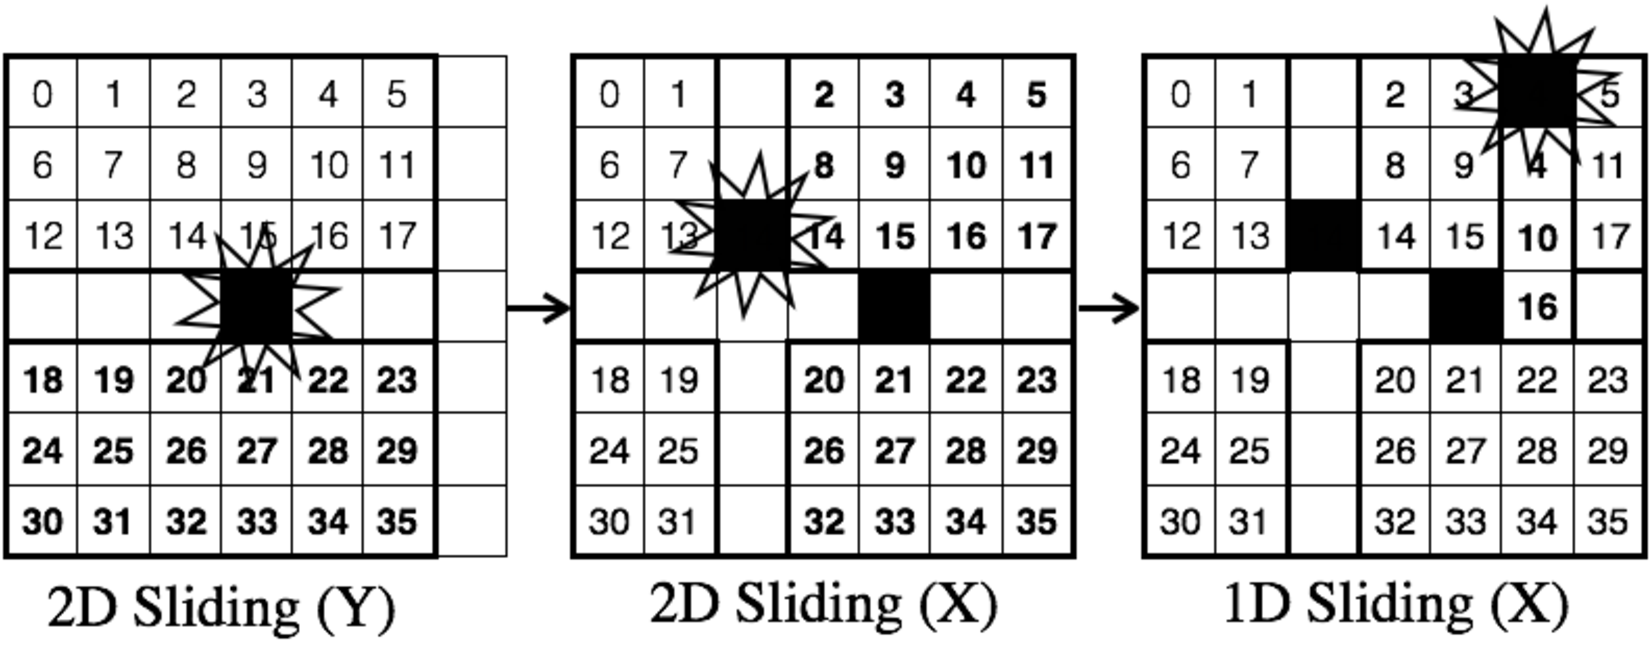
\includegraphics[width=0.95\columnwidth]{Figs/HybridSliding.pdf}
  \caption{Hybrid Sliding Methods}
  \label{fig:hybrid-methods}
\end{center}
\end{figure}

Those substitution methods can be combined and this is named {\sl
hybrid sliding} method as shown in Figure~\ref{fig:hybrid-methods}. In
this hybrid sliding method, the method having the highest order must
be applied. And if the sliding method cannot be applied, then the
lower order sliding method is applied. Since the 0D sliding method has no
limitation as long as spare nodes exits, it can be used as a last resort.

We developed a simulator of the proposed sliding methods to count the 
maximum message collisions and evaluated it on the K computer, BG/Q
and Tsubame2.5\cite{Hori:2015:SSF:2802658.2802670}. 

\section{Subsequent Development}

Although this project was started with the prediction of
heterogeneous CPU architecture would be a common many-core
architecture, this does not come true. Intel announced standalone
many-core CPU, Knights Landing (KNL). Still, GP-GPUs are not
standalone and require host CPU, however, most GP-GPUs are black-box
from the viewpoint of OS and only little things can be done with
them. Although MPVAS software developed in this project became
useless, the idea of packing multiple processes into one virtual
address space is still effective.

The PVAS project is still active. One of the most drawback of PVAS was
the implementation by the patched Linux and PVAS was hard to port to the
other OSes and architectures. To overcome this, a new
user-level implementation has been being developed, named
Process-in-Process (PiP). 
The other techniques developed in this project excepting MPVAS are
applicable for the exa-scale computing. The research on scalable
MPI-IO, EARTH, is going on. The ULFM development team is
trying to push ULFM into the MPI standard.

\section{Summary}
